\usepackage{xcolor}
\usepackage{afterpage}
\usepackage{pifont,mdframed}
\usepackage[bottom]{footmisc}
\usepackage{multicol}

\createsection{\Grader}{Grader di prova}
\createsection{\Detail}{Dettagli}

\renewcommand{\inputfile}{\texttt{stdin}}
\renewcommand{\outputfile}{\texttt{stdout}}
\makeatletter
\renewcommand{\this@inputfilename}{\texttt{stdin}}
\renewcommand{\this@outputfilename}{\texttt{stdout}}
\makeatother

\newenvironment{warning}
  {\par\begin{mdframed}[linewidth=2pt,linecolor=gray]%
    \begin{list}{}{\leftmargin=1cm
                   \labelwidth=\leftmargin}\item[\Large\ding{43}]}
  {\end{list}\end{mdframed}\par}
\newenvironment{danger}
{\par\begin{mdframed}[linewidth=2pt,linecolor=red!60!yellow,backgroundcolor=red!20!white]%
		\begin{list}{}{\leftmargin=1cm
				\labelwidth=\leftmargin}\item[\Large\ding{45}]}
		{\end{list}\end{mdframed}\par}

% % % % % % % % % % % % % % % % % % % % % % % % % % % % % % % % % % % % % % % % % % %
% % % % % % % % % % % % % % % % % % % % % % % % % % % % % % % % % % % % % % % % % % %

After the competition, the $P$ participants of the Italian Olympiad in
Informatics (labeled from $0$ to $P-1$) will attend the gala dinner, in
a traditional Molise fashion.

The banquet consists of $S$ plates labeled from $0$ to $S-1$, each plate
containing one of the ``100 best Molise delicacies'' personally chosen by the
chef: \emph{composta molisana}, \emph{spezzatino di pecora},
\emph{agnello con cicoria} and other $97$ typical dishes from Molise.

Once at the gala dinner, the participants will head towards the beginning of the
buffet, going from right to left (from plate $S-1$ to plate $0$) and
they will choose to either sit down or skip to the next plate. Each participant
has a favorite dish, so he/she will sit down only in one of the spots where
his/her favorite dish is served. The participants will arrive at the banquet in
the same order they were ranked in the contest.

It is not allowed to climb over others, so when a participant
chooses to sit down in front of the $i$-th plate, then all the plates in
positions $j < i$ will be unreachable to the following participants. Once seated, the
participants will keep the same order in which they arrived. It is possible to
have ``empty spots'' where no one is seated. The participants don't necessarily
need to choose the first ``favorite'' dish they see on the table: \emph{they can
choose any plate} among those containing their favorite dish, as shown below.

\begin{figure}[H]%
	\centering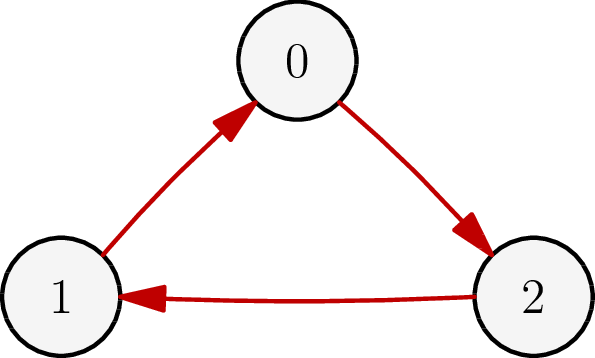
\includegraphics[width=\linewidth]{asy_cena/fig1.pdf}
\end{figure}

Unfortunately there is a problem! Mojito and Chupito, Monica's dog and cat
respectively, escaped her sight and entered the banquet room before the
participants' arrival. The two brats jumped on the long table with the intent of
eating some of the dishes:
\begin{itemize}[nolistsep]
	\item Mojito jumped on the \emph{left} side of the table, to eat plates
  starting from the $0$-th.
	\item Chupito jumped on the \emph{right} side of the table, to eat plates
  starting from the $(S-1)$-th.
\end{itemize}

Monica, realizing that her pets were missing, quickly ran to the buffet and now
she has to choose how and when to stop them. It is possible to stop Mojito and
Chupito at any point, even before they start to eat. However, touched by the cute
fluffiness of her puppies, Monica would like to let them eat for a while. Of course,
she should make sure that there's still food for the contestants.

Let's denote with $A$ and $B$ respectively the number of dishes eaten by Mojito
and by Chupito. Compute \textbf{how many different pairs} $(A, B)$ exist such
that, even ``sacrificing'' the first $A$ and the last $B$ plates of the
table, \textbf{there exists at least a strategy} that allows the participants to
all sit down in front of a plate containing their favorite dish.

\begin{danger}
	\textbf{Important:} participants are curious to try Molise delicacies. Thus,
  	regardless of the value of $P$, the number of participants \emph{with the
  	same favorite dish} is not greater than \textbf{1000}.
\end{danger}

% % % % % % % % % % % % % % % % % % % % % % % % % % % % % % % % % % % % % % % % % % %
% % % % % % % % % % % % % % % % % % % % % % % % % % % % % % % % % % % % % % % % % % %

\Implementation

You should submit only one file, with extension \texttt{.c} or \texttt{.cpp}.

\begin{warning}
  Among the attachments of this task you will find a template \texttt{cena.c}
  and \texttt{cena.cpp} with an example of implementation.
\end{warning}

You have to implement the following function:

\begin{center}\begin{tabularx}{\textwidth}{|c|X|}
\hline
C/C++  & \verb|long long conta(int S, int s[], int P, int p[]);|\\
\hline
\end{tabularx}\end{center}

\begin{itemize}[nolistsep]
  \item The integer $S$ is the number of plates on the table.
  \item The array $s$ (indexed from $0$ to $S-1$) specifies the type of food for the $i$-th plate.
  \item The integer $P$ is the number of participants.
  \item The array $p$ (indexed from $0$ to $P-1$) specifies the preference of the $i$-th participant.
\end{itemize}

The grader will call the function \texttt{conta} and will print the returned
value in the output file.

% % % % % % % % % % % % % % % % % % % % % % % % % % % % % % % % % % % % % % % % % % %
% % % % % % % % % % % % % % % % % % % % % % % % % % % % % % % % % % % % % % % % % % %


\Grader
In the directory of this problem there is a simplified version of the grader
used during evaluation, that you can use to test your solutions locally. The
sample grader reads data from \inputfile{}, calls the functions that you have to
implement and writes in \outputfile{}.

The input file is formed by three lines:
\begin{itemize}[nolistsep,itemsep=2mm]
\item Line $1$: integers $S$ and $P$.
\item Line $2$: values \texttt{s[$i$]} for $i = 0\ldots S-1$.
\item Line $3$: values \texttt{p[$i$]} for $i = 0\ldots P-1$.
\end{itemize}

Output file is formed by just one line, containing:
\begin{itemize}[nolistsep,itemsep=2mm]
\item Line $1$: the value returned by function \texttt{conta}.
\end{itemize}

% % % % % % % % % % % % % % % % % % % % % % % % % % % % % % % % % % % % % % % % % % %
% % % % % % % % % % % % % % % % % % % % % % % % % % % % % % % % % % % % % % % % % % %


\Constraints

\begin{itemize}[nolistsep, itemsep=2mm]
	\item $1 \le P \le S \le 100\,000$.
	\item $1 \le P \le 50\,000$.
	\item $0 \le \texttt{s[$i$]}, \texttt{p[$i$]} < 100$.
	\item There aren't $1001$ participants with the same preference.
\end{itemize}

% % % % % % % % % % % % % % % % % % % % % % % % % % % % % % % % % % % % % % % % % % %
% % % % % % % % % % % % % % % % % % % % % % % % % % % % % % % % % % % % % % % % % % %


\Scoring

Your program will be tested on several test cases grouped in subtask. To
achieve the score of a subtask, you need to correctly solve all of its test cases.

\begin{itemize}[nolistsep,itemsep=2mm]
  \item \textbf{\makebox[2cm][l]{Subtask 1} [\phantom{1}0 points]}: Sample cases.
  \item \textbf{\makebox[2cm][l]{Subtask 2} [13 points]}: $S \leq 100$ and $P\le 100$. % O(S³)
  \item \textbf{\makebox[2cm][l]{Subtask 3} [23 points]}: $P\le 1000$ and all the participants have the same preference.
  \item \textbf{\makebox[2cm][l]{Subtask 4} [27 points]}: $S \leq 10\,000$ and $P \le 100$. % O(S²P)
  \item \textbf{\makebox[2cm][l]{Subtask 5} [16 points]}: $P\le 100$. % O(SP)
  \item \textbf{\makebox[2cm][l]{Subtask 6} [21 points]}: No additional limitations. % O(SA)
\end{itemize}

% % % % % % % % % % % % % % % % % % % % % % % % % % % % % % % % % % % % % % % % % % %
% % % % % % % % % % % % % % % % % % % % % % % % % % % % % % % % % % % % % % % % % % %


\Examples

\begin{example}
\exmpfile{cena.input0.txt}{cena.output0.txt}%
\exmpfile{cena.input1.txt}{cena.output1.txt}%
\end{example}

% % % % % % % % % % % % % % % % % % % % % % % % % % % % % % % % % % % % % % % % % % %
% % % % % % % % % % % % % % % % % % % % % % % % % % % % % % % % % % % % % % % % % % %


\Explanation

The \textbf{first sample case} is the one illustrated in the task description.
To guarantee a sitting strategy for all participants, there are $4$ possible
ways to stop Mojito and Chupito.

\begin{itemize}[nolistsep,itemsep=2mm]
	\item \texttt{0[\underline{0}1\underline{2}\underline{0}]1} -- Monica lets Mojito eat $1$ dish and Chupito eat $1$ dish.
	\item \texttt{[0\underline{0}1\underline{2}\underline{0}1]} -- Mojito $0$ dishes, Chupito $0$ dishes.
	\item \texttt{[\underline{0}01\underline{2}\underline{0}]1} -- Mojito $0$ dishes, Chupito $1$ dish.
	\item \texttt{0[\underline{0}1\underline{2}\underline{0}1]} -- Mojito $1$ dish, Chupito $0$ dishes.
\end{itemize}

The table area which hasn't been touched by the two hungry pets is indicated
between square brackets. Also, to show that all these ways guarantee a sitting
strategy for participants, a possible disposition of the participants is underlined.

In the \textbf{second sample case} all participants have the same preference,
any way to stop Mojito and Chupito that leaves at least $3$ plates of type
\texttt{`0'} is thus valid.

\setlength{\columnsep}{-2.1in}
\begin{multicols}{2}
	\begin{itemize}[nolistsep,itemsep=2mm]
		\item \texttt{[\underline{0}1\underline{0}11\underline{0}]101}
		\item \texttt{[\underline{0}1\underline{0}11\underline{0}1]01}
		\item \texttt{[01\underline{0}11\underline{0}1\underline{0}]1}
		\item \texttt{[\underline{0}1011\underline{0}1\underline{0}1]}

		\item \texttt{0[1\underline{0}11\underline{0}1\underline{0}]1}
		\item \texttt{0[1\underline{0}11\underline{0}1\underline{0}1]}
		\item \texttt{01[\underline{0}11\underline{0}1\underline{0}]1}
		\item \texttt{01[\underline{0}11\underline{0}1\underline{0}1]}
	\end{itemize}
\end{multicols}
